%----- Automatically generated by TTool version 0.99 generation date: 12/07/2022 16:35----

\section{Analysis}
\subsection{System\_UseCase}
Figures \ref{fig:SystemUseCaseSystemUseCase00} presents ...
\begin{figure*}[htb]
\centering
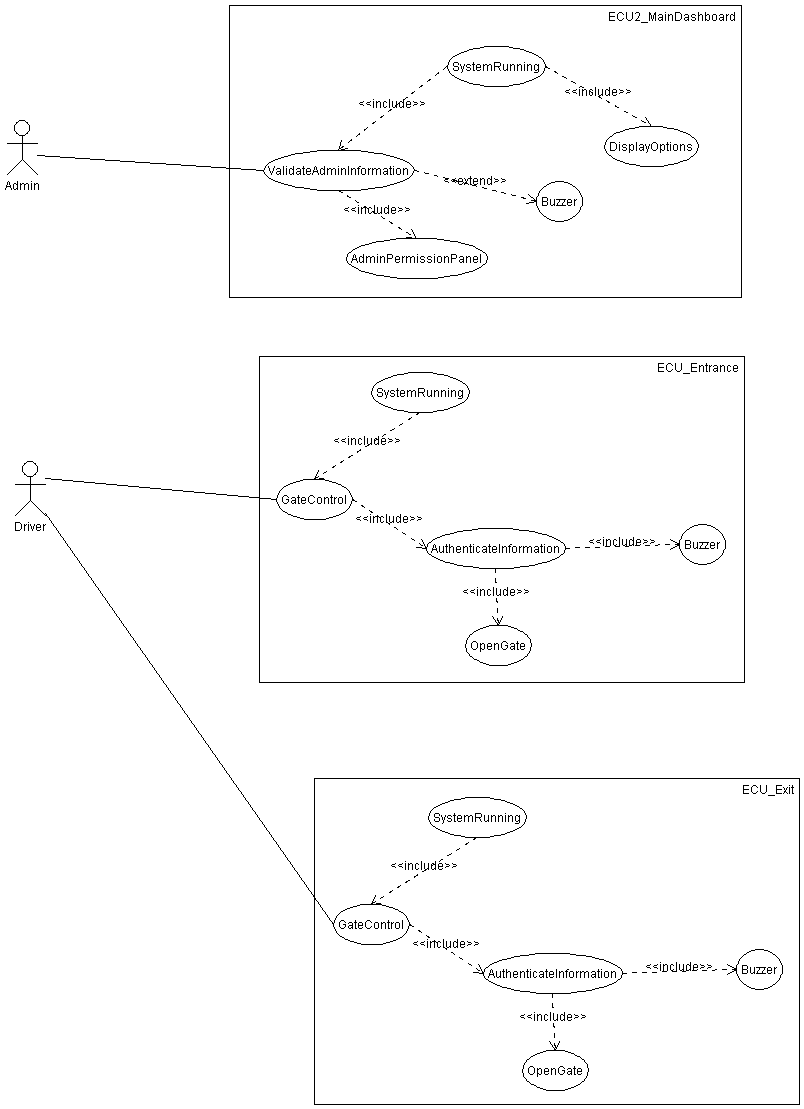
\includegraphics[width=\textwidth]{img_0_0.png}
\caption{Diagram "System\_UseCase"}
\label{fig:SystemUseCaseSystemUseCase00}
\end{figure*}

\subsection{ECU2\_Dashboard\_ActivityDiagram}
Figures \ref{fig:ECU2DashboardActivityDiagramECU2DashboardActivityDiagram01} presents ...
\begin{figure*}[htb]
\centering
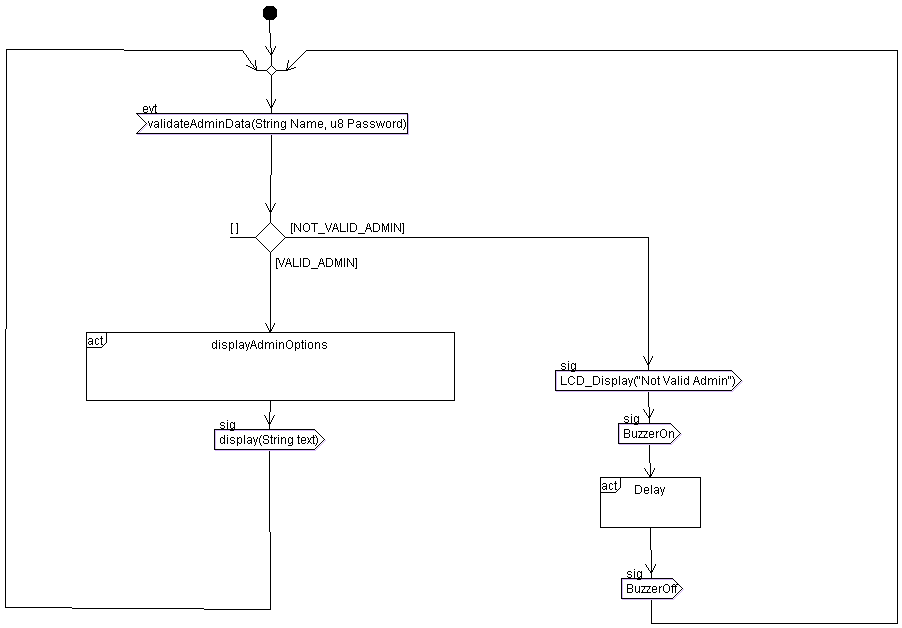
\includegraphics[width=\textwidth]{img_0_1.png}
\caption{Diagram "ECU2\_Dashboard\_ActivityDiagram"}
\label{fig:ECU2DashboardActivityDiagramECU2DashboardActivityDiagram01}
\end{figure*}

\subsection{ECU3\_Entrance\_ActivityDiagram}
Figures \ref{fig:ECU3EntranceActivityDiagramECU3EntranceActivityDiagram02} presents ...
\begin{figure*}[htb]
\centering
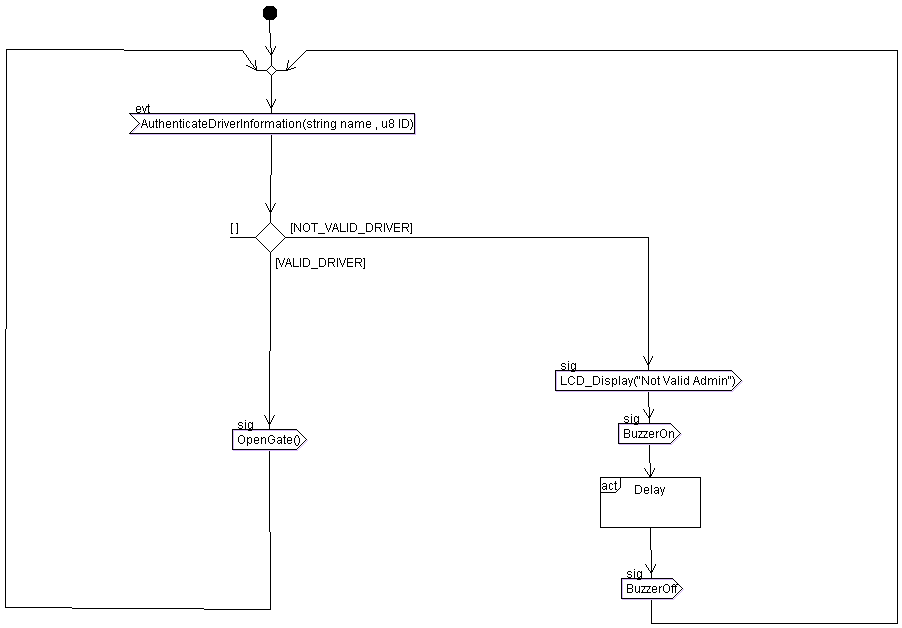
\includegraphics[width=\textwidth]{img_0_2.png}
\caption{Diagram "ECU3\_Entrance\_ActivityDiagram"}
\label{fig:ECU3EntranceActivityDiagramECU3EntranceActivityDiagram02}
\end{figure*}

\subsection{ECU3\_Exit\_ActivityDiagram}
Figures \ref{fig:ECU3ExitActivityDiagramECU3ExitActivityDiagram03} presents ...
\begin{figure*}[htb]
\centering
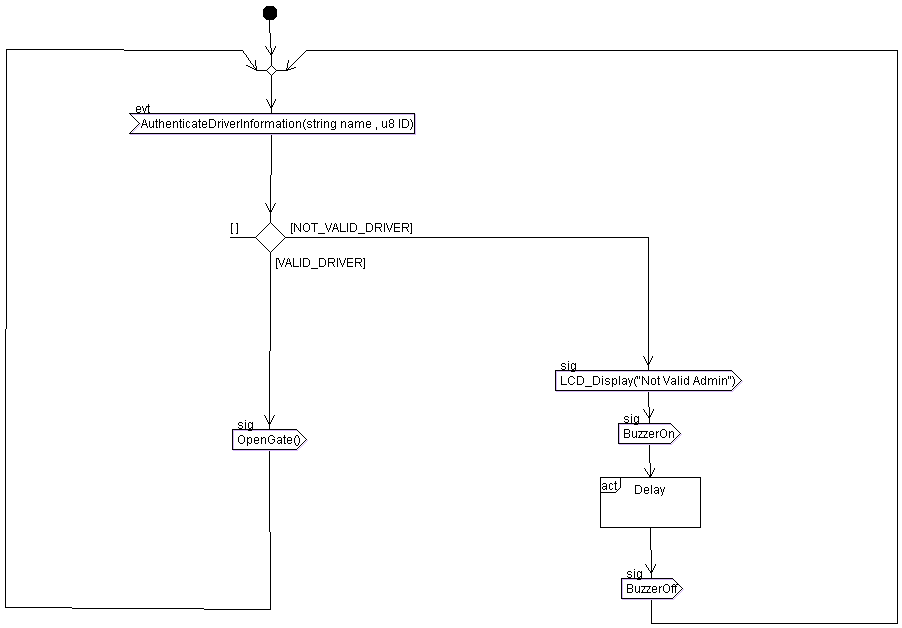
\includegraphics[width=\textwidth]{img_0_3.png}
\caption{Diagram "ECU3\_Exit\_ActivityDiagram"}
\label{fig:ECU3ExitActivityDiagramECU3ExitActivityDiagram03}
\end{figure*}

\subsection{Sytem\_SeqDiagram}
Figures \ref{fig:SytemSeqDiagramSytemSeqDiagram04} presents ...
\begin{figure*}[htb]
\centering
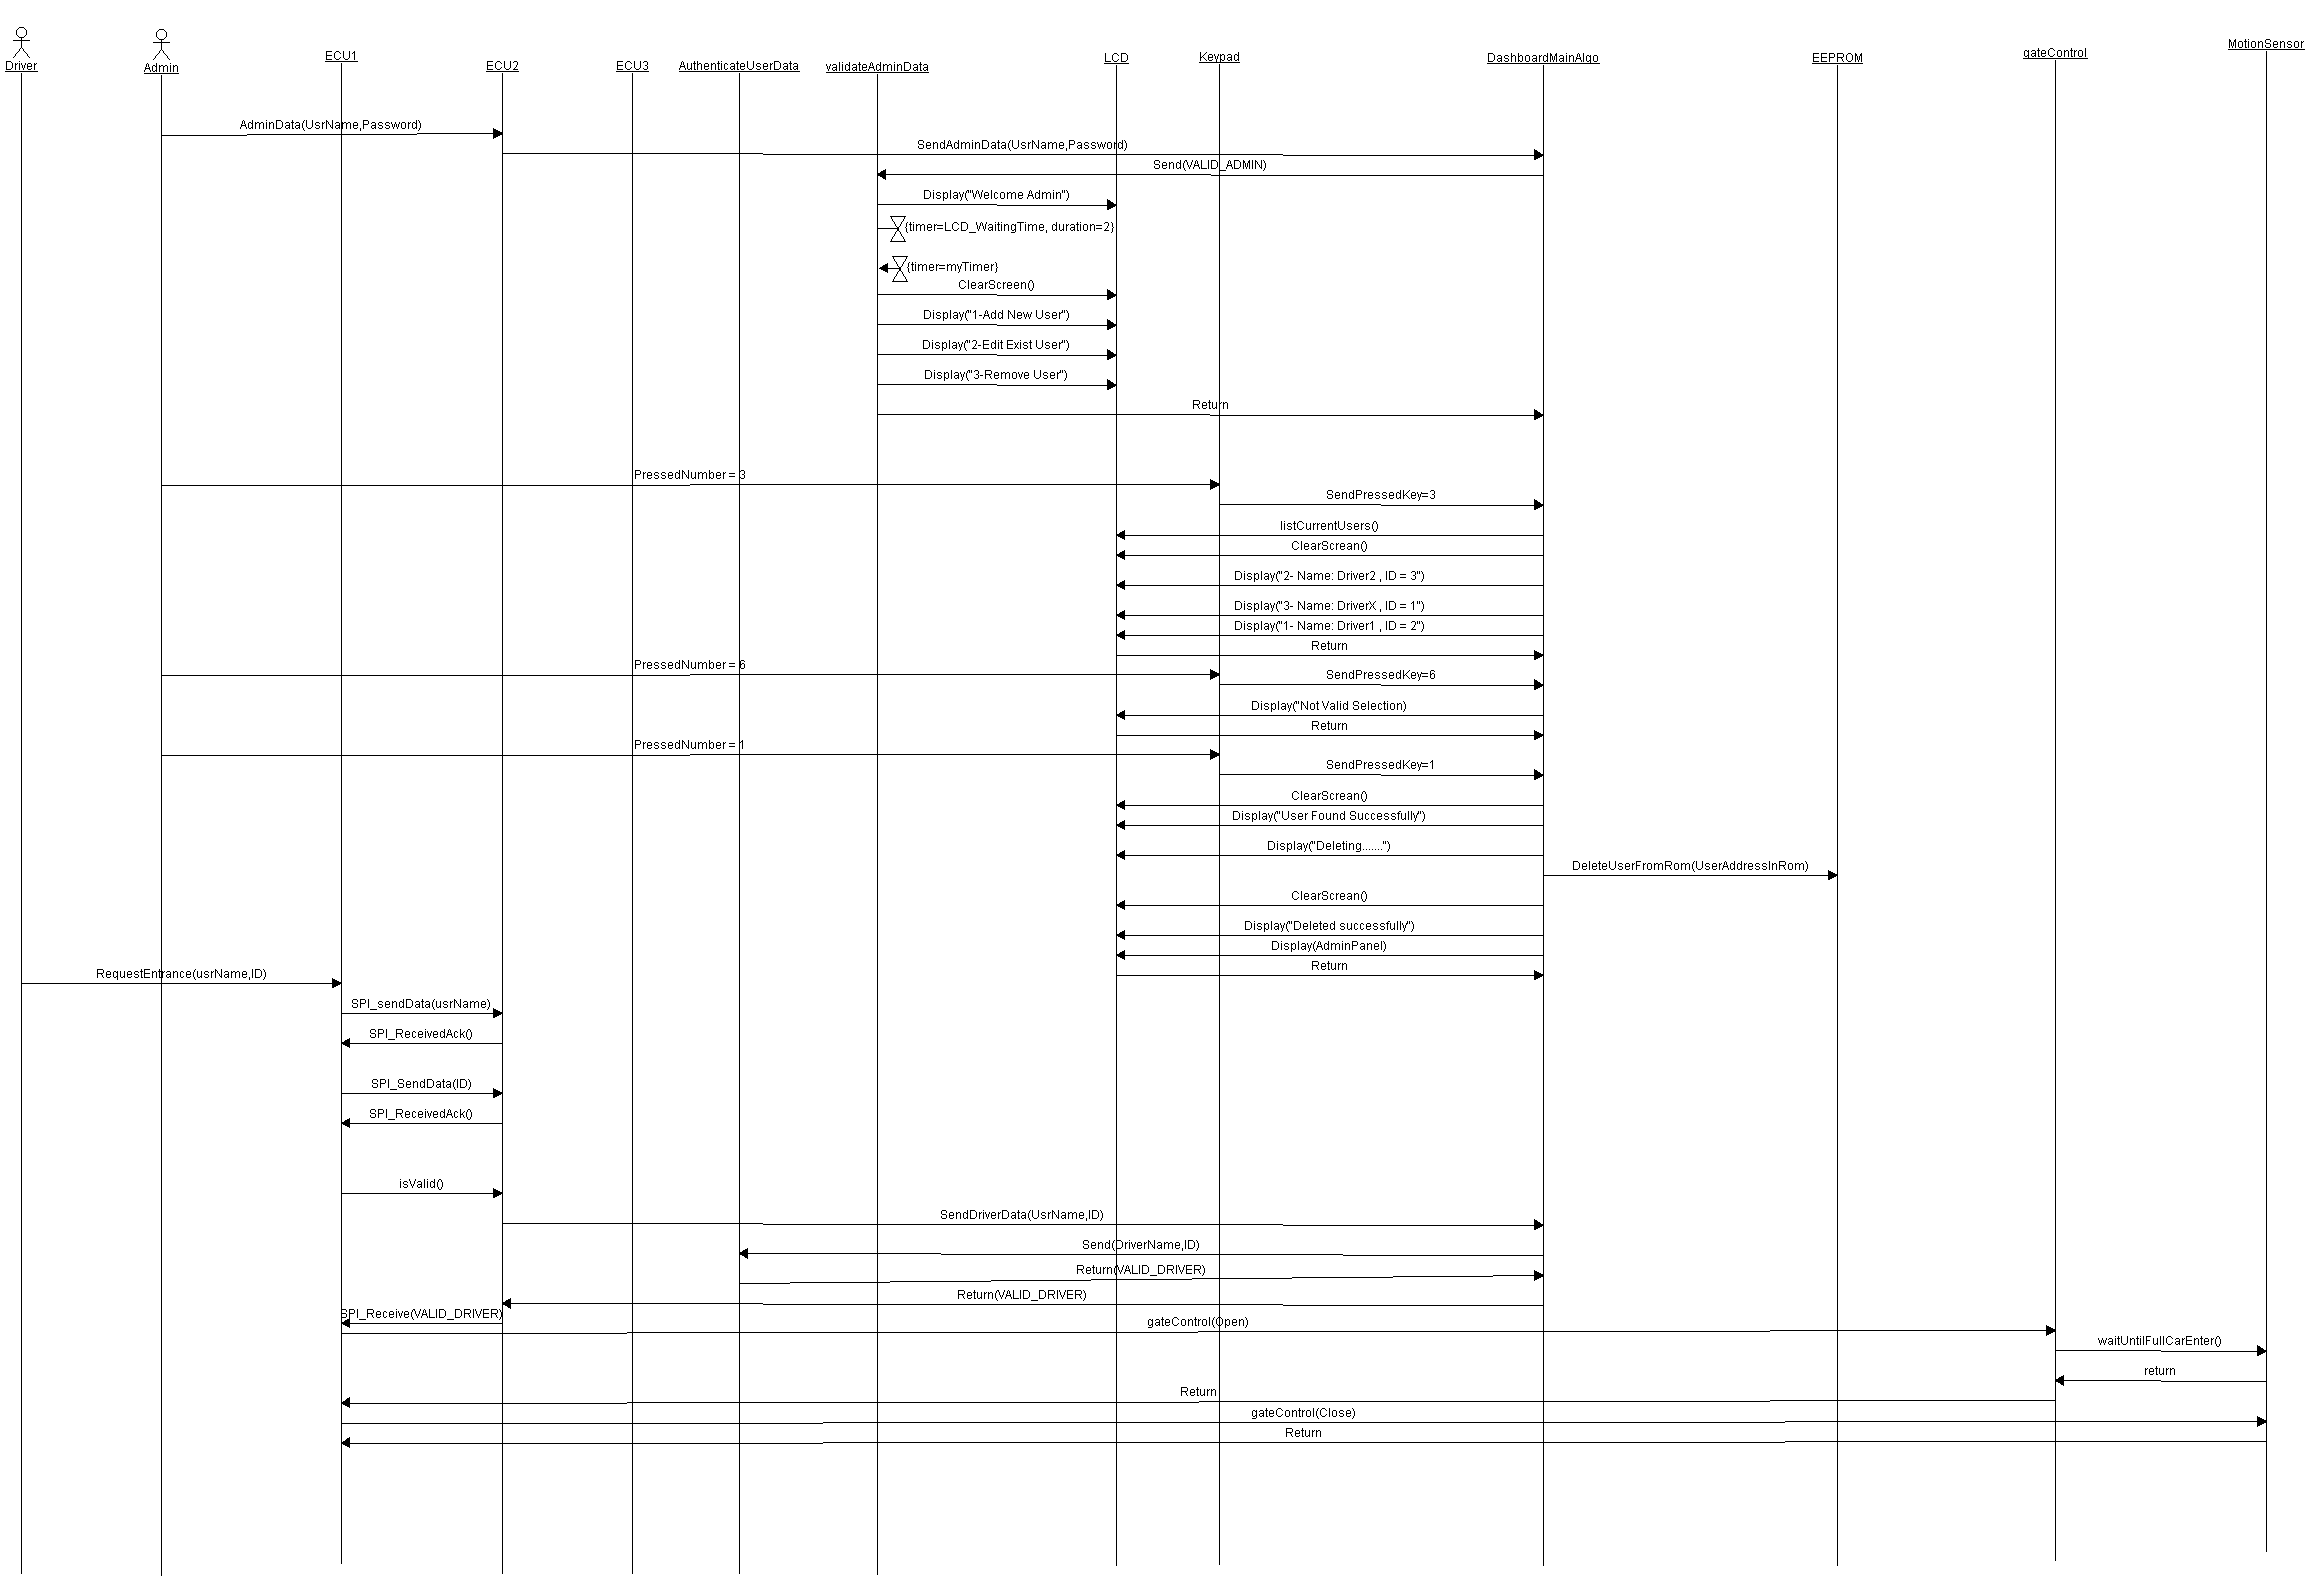
\includegraphics[width=\textwidth]{img_0_4.png}
\caption{Diagram "Sytem\_SeqDiagram"}
\label{fig:SytemSeqDiagramSytemSeqDiagram04}
\end{figure*}

\section{Requirements}
\subsection{AVATAR RD}
Figures \ref{fig:AVATAR RDAVATAR RD10} presents ...
\begin{figure*}[htb]
\centering
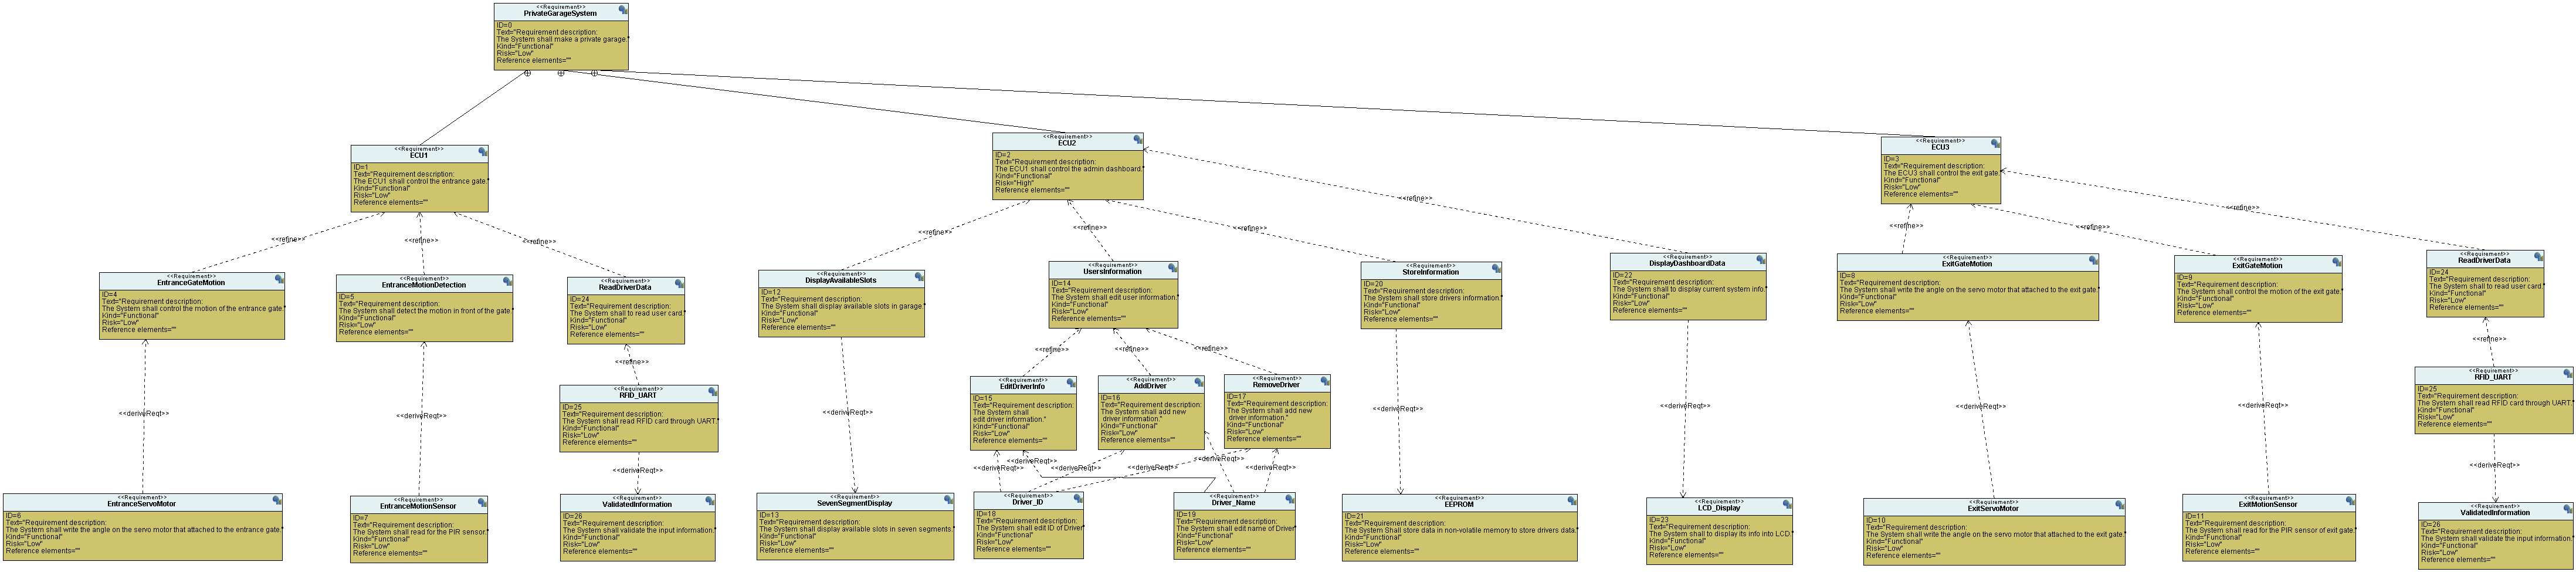
\includegraphics[width=\textwidth]{img_1_0.png}
\caption{Diagram "AVATAR RD"}
\label{fig:AVATAR RDAVATAR RD10}
\end{figure*}

\section{Design}
\subsection{Block Diagram}
Figures \ref{fig:Block DiagramBlock Diagram20} presents ...
\begin{figure*}[htb]
\centering
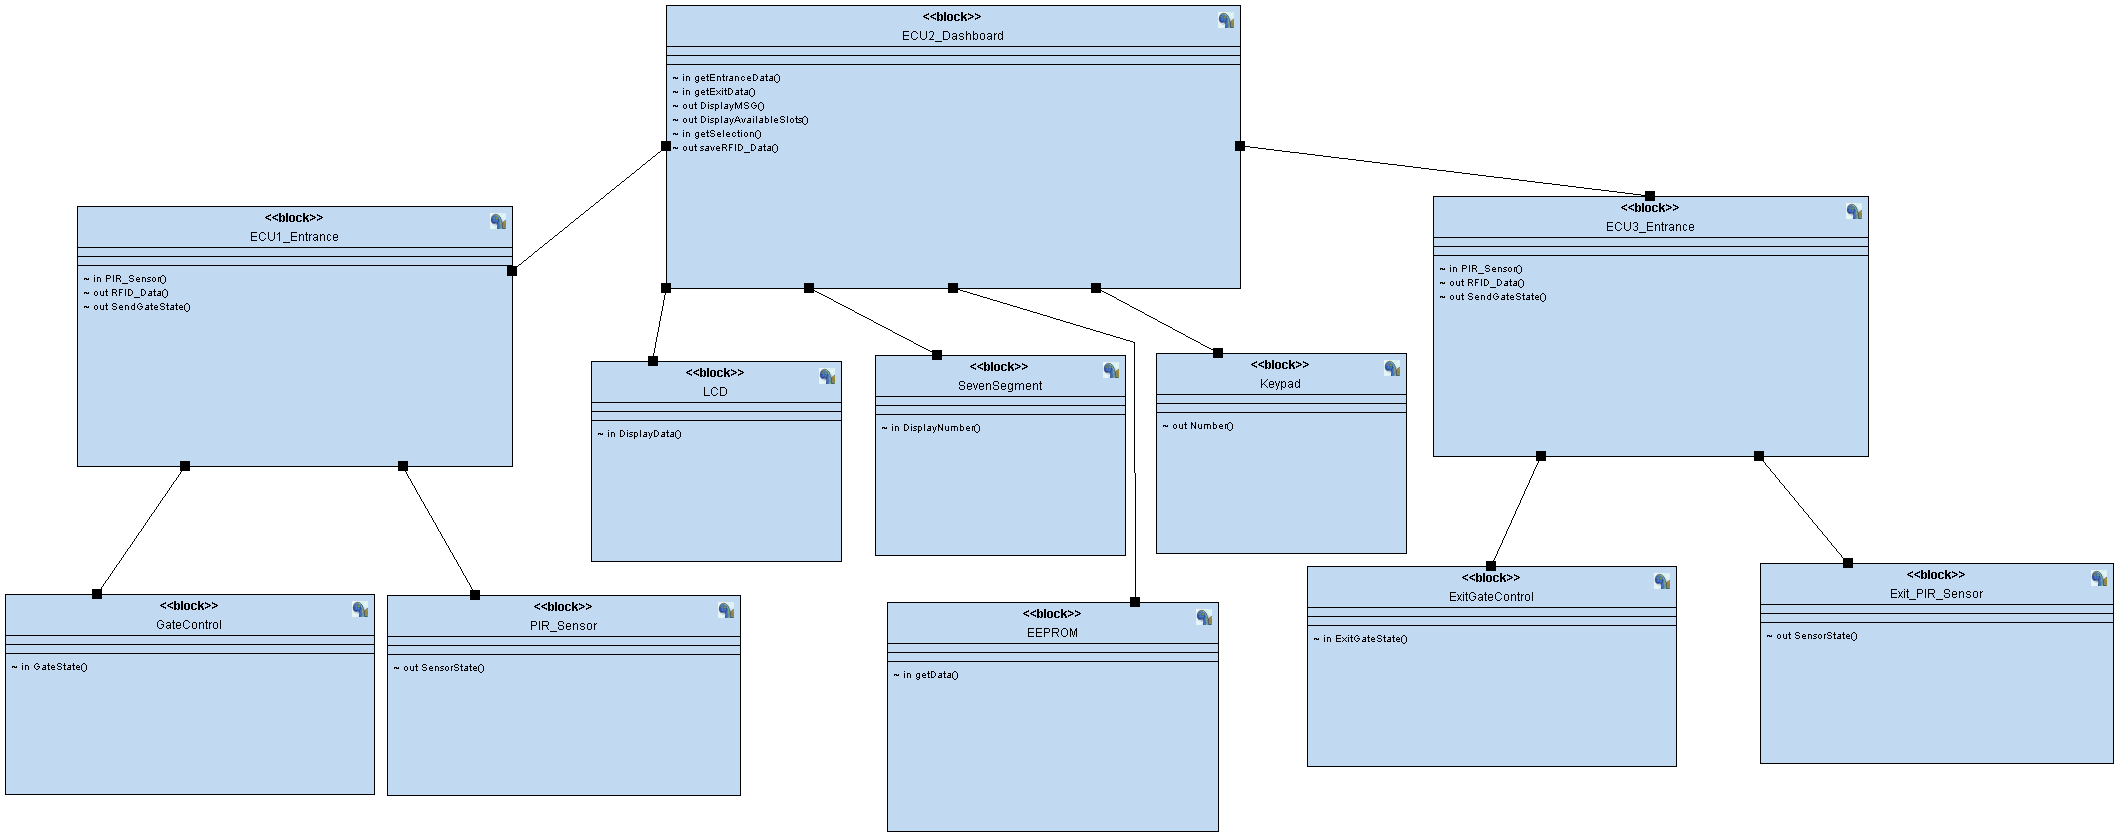
\includegraphics[width=\textwidth]{img_2_0.png}
\caption{Diagram "Block Diagram"}
\label{fig:Block DiagramBlock Diagram20}
\end{figure*}

\subsection{Behavior of Block: EEPROM}
Figures \ref{fig:EEPROMEEPROM21} presents ...
\begin{figure*}[htb]
\centering
\includegraphics[width=\textwidth]{img_2_1.png}
\caption{Diagram "Behavior of Block: EEPROM"}
\label{fig:EEPROMEEPROM21}
\end{figure*}

\subsection{Behavior of Block: Keypad}
Figures \ref{fig:KeypadKeypad22} presents ...
\begin{figure*}[htb]
\centering
\includegraphics[width=\textwidth]{img_2_2.png}
\caption{Diagram "Behavior of Block: Keypad"}
\label{fig:KeypadKeypad22}
\end{figure*}

\subsection{Behavior of Block: SevenSegment}
Figures \ref{fig:SevenSegmentSevenSegment23} presents ...
\begin{figure*}[htb]
\centering
\includegraphics[width=\textwidth]{img_2_3.png}
\caption{Diagram "Behavior of Block: SevenSegment"}
\label{fig:SevenSegmentSevenSegment23}
\end{figure*}

\subsection{Behavior of Block: LCD}
Figures \ref{fig:LCDLCD24} presents ...
\begin{figure*}[htb]
\centering
\includegraphics[width=\textwidth]{img_2_4.png}
\caption{Diagram "Behavior of Block: LCD"}
\label{fig:LCDLCD24}
\end{figure*}

\subsection{Behavior of Block: PIR\_Sensor}
Figures \ref{fig:PIRSensorPIRSensor25} presents ...
\begin{figure*}[htb]
\centering
\includegraphics[width=\textwidth]{img_2_5.png}
\caption{Diagram "Behavior of Block: PIR\_Sensor"}
\label{fig:PIRSensorPIRSensor25}
\end{figure*}

\subsection{Behavior of Block: ECU1\_Entrance}
Figures \ref{fig:ECU1EntranceECU1Entrance26} presents ...
\begin{figure*}[htb]
\centering
\includegraphics[width=\textwidth]{img_2_6.png}
\caption{Diagram "Behavior of Block: ECU1\_Entrance"}
\label{fig:ECU1EntranceECU1Entrance26}
\end{figure*}

\subsection{Behavior of Block: ECU2\_Dashboard}
Figures \ref{fig:ECU2DashboardECU2Dashboard27} presents ...
\begin{figure*}[htb]
\centering
\includegraphics[width=\textwidth]{img_2_7.png}
\caption{Diagram "Behavior of Block: ECU2\_Dashboard"}
\label{fig:ECU2DashboardECU2Dashboard27}
\end{figure*}

\subsection{Behavior of Block: Exit\_PIR\_Sensor}
Figures \ref{fig:ExitPIRSensorExitPIRSensor28} presents ...
\begin{figure*}[htb]
\centering
\includegraphics[width=\textwidth]{img_2_8.png}
\caption{Diagram "Behavior of Block: Exit\_PIR\_Sensor"}
\label{fig:ExitPIRSensorExitPIRSensor28}
\end{figure*}

\subsection{Behavior of Block: ECU3\_Entrance}
Figures \ref{fig:ECU3EntranceECU3Entrance29} presents ...
\begin{figure*}[htb]
\centering
\includegraphics[width=\textwidth]{img_2_9.png}
\caption{Diagram "Behavior of Block: ECU3\_Entrance"}
\label{fig:ECU3EntranceECU3Entrance29}
\end{figure*}

\subsection{Behavior of Block: ExitGateControl}
Figures \ref{fig:ExitGateControlExitGateControl210} presents ...
\begin{figure*}[htb]
\centering
\includegraphics[width=\textwidth]{img_2_10.png}
\caption{Diagram "Behavior of Block: ExitGateControl"}
\label{fig:ExitGateControlExitGateControl210}
\end{figure*}

\subsection{Behavior of Block: GateControl}
Figures \ref{fig:GateControlGateControl211} presents ...
\begin{figure*}[htb]
\centering
\includegraphics[width=\textwidth]{img_2_11.png}
\caption{Diagram "Behavior of Block: GateControl"}
\label{fig:GateControlGateControl211}
\end{figure*}

